\part{}
\chapter{Design}
\section{Design Process}
The typical design process is shown in \figref{fig:design_flow}.
\begin{figure}[p]
\centering
\begin{tikzpicture}[scale=1,auto,node distance=1.9cm,line/.style={draw,thick,-latex'},background rectangle/.style={fill=exmpbg},show background rectangle]
\begin{scope}[every node/.style={text centered,rectangle,rounded corners,draw=black,inner sep=8pt},every path/.style=line]
\node(need){NEED};
\node(concept)[below=1.5cm of need]{CONCEPT};
\node(analysis)[below=5cm of concept]{ANALYSIS};
\node(force)[above left=1.5cm and 1cm of analysis.center]{FORCES};
\node(member)[text width=3cm,above right=1.5cm and 1cm of analysis.center]{MEMBER PROPERTIES};
\node(material)[text width=3cm,above=.5cm of member]{MATERIAL PROPERTIES};
\node(selection)[below of=analysis]{SELECTION};
\node(modification)[below of=selection]{MODIFICATION};
\node(presentation)[below of=modification]{PRESENTATION};
\node(approval)[below of=presentation]{APPROVAL};
\node(production)[below of=approval]{PRODUCTION};
\node(contracting)[below of=production]{CONTRACTING};
\node(overseeing)[below of=contracting]{OVERSEEING};
\path(need)--(concept);
\path(concept)--(analysis);
\path(analysis)--(selection);
\path(selection)--(modification);
\path(modification)--(presentation);
\path(presentation)--(approval);
\path(approval)--(production);
\path(production)--(contracting);
\path(contracting)--(overseeing);
\draw(modification.east)--++(.5,0)|-(analysis.east);
\path(material)--(member);
\draw(member.south)|-($(analysis.north)+(0,4mm)$);
\draw(force.south)|-($(analysis.north)+(0,4mm)$);
\end{scope}
\begin{scope}[every node/.style={text width=8cm,inner sep=8pt}]
\node(exp.need)[right=4cm of need.center]{basic need to cover, support, span, transport, contain, etc. (government organization or company)};
\node(exp.concept)[right=4cm of concept.center]{initial idealization of structural type based on knowledge of materials, approximate loads, structural behavior, experience and geometric requirements (engineer or architect)};
\node(exp.analysis)[right=4cm of analysis.center]{calculation of member forces};
\node(exp.selection)[right=4cm of selection.center]{selection of member sizes, details, etc.};
\node(exp.modification)[right=4cm of modification.center]{based on requirement changes, material availability, coordination with other planners (caused by client, architect, industry, heating and ventilating people, etc.)};
\node(exp.presentation)[right=4cm of presentation.center]{clear construction drawings};
\node(exp.approval)[right=4cm of approval.center]{verification with client that the structure satisfies needs};
\node(exp.production)[right=4cm of production.center]{production of final construction documents};
\node(exp.contracting)[right=4cm of contracting.center]{letting contract};
\node(exp.overseeing)[right=4cm of overseeing.center]{checking that structure is built according to specification and solving site problems};
\end{scope}
\end{tikzpicture}
\caption{Typical design process}\label{fig:design_flow}
\end{figure}
\section{Design Approaches}
\subsection{Design for Strength}
The ultimate requirement can be summarised by the following inequality:
\begin{gather}
\parbox{5cm}{\bfseries\centering{}FORCE DEMAND\\(ACTIONS, LOADS)}\leqslant\parbox{6cm}{\bfseries\centering{}STRENGTH\\(CAPACITY, RESISTANCE)}
\end{gather}

There are two common design methods for this strength requirement.
\subsubsection{ASD}
It stands for \textbf{Working Stress (or Allowable Stress) Design (ASD)} (e.g., NZ Steel Codes pre-1984).
\begin{align*}
\sum\parbox{2cm}{\bfseries\centering{}WORKING\\FORCES}&\leqslant\parbox{3cm}{\bfseries\centering{}PERMISSIBLE\\STRENGTH},\\[4mm]
\sum{}E_i&\leqslant\dfrac{\text{Ultimate Strength}}{\text{Safety Factor}}=\dfrac{R}{\text{SF}}.
\end{align*}

The safety factor, SF is approximately equal to \num{1.7} and it allows for variation in loading and material strength. ASD was popular in NZ until the mid 1980s. In the USA, and some other countries, it is still used, especially for timber, and for some steel structures. It assumes that all types of loading have the same weighting. It cannot handle unusual loads well.
\subsubsection{LSD, LRFD}
It stands for \textbf{Limit State Design, a.k.a., Load and Resistance Factor Design (LRFD)} (e.g., many NZ Steel Codes post-1984).

A structure should be designed in such a way that it does not reach a \textbf{critical limit state}.
\begin{gather*}
\text{\bfseries{}structural state}\leqslant\text{\bfseries{}limit state}
\end{gather*}

A critical limit state for a structure may be governed by the following aspects:
\begin{itemize}
\item safety
\begin{itemize}
\item strength
\item stability
\end{itemize}
\item serviceability
\begin{itemize}
\item deformation
\item vibration
\end{itemize}
\end{itemize}

NZ limit state design codes are written in a LRFD format recognizing the probabilistic variations in both applied forces and capacities.

The many advantages of LRFD are well--expressed by Beedle, whose listing is the basis of the following:
\begin{mdframed}[style=highlight]
\begin{enumerate}
\item LRFD is another `tool' for structural engineers to use in steel design. Why not have the same tools (variable overload factors and resistance factors) available for steel design as are available for concrete design?
\item Adoption of LRFD is not mandatory but provides a flexibility of options to the designer. The marketplace will dictate whether or not LRFD will become the sole method.
\item ASD is an approximate way to account for what LRFD does in a more rational way. The use of plastic design concepts in ASD has made ASD such that it no longer may be called an `elastic design' method.
\item The rationality of LRFD has always been attractive, and becomes an incentive permitting the better and more economical use of material for some load combinations and structural configurations. It will also likely lead to having safer structures in view of the arbitrary practice under ASD of combining dead and live loads and treating them the same.
\item Using multiple load factor combinations should lead to economy.
\item LRFD will facilitate the input of new information on loads and load variations as such information becomes available. Considerable knowledge of the resistance of steel structures is available. On the other hand our knowledge of loads and their variation is much less. Separating the loading from the resistance allows one to be changed without the other if that should be desired.
\item Changes in overload factors and resistance factors $\phi$ are much easier to make than to change the allowable stress in ASD.
\item LRFD makes design in all materials more compatible. The variability of loads is actually unrelated to the material used in the design. Future specifications not in the limit states format for any material will put that material at a disadvantage in design.
\item LRFD provides the framework to handle unusual loads that may not be covered by the specification. The design may have uncertainty relating to the resistance of the structure, in which case the resistance factors may be modified. On the other hand, the uncertainty may relate to the loads and different overload factors may be used.
\item Future adjustments in the calibration of the method can be made without much complication. Calibration for LRFD was done for an \textit{average} situation but might be adjusted in the future.
\item Economy is likely to result for low live load to dead load ratios. For high live load to dead load ratios there will be diseconomy but a low amount.
\item Safer structures may result under LRFD because the method should lead to a better awareness of structural behaviour.
\end{enumerate}
\end{mdframed}

LRFD equation has the following typical form:
\begin{align}
\sum\gamma_iE_i&\leqslant\phi{}R_n,\\
\text{\textbf{Forces}}&\leqslant\text{\textbf{Resistance}},
\end{align}
where
\begin{conditions}
\gamma_i&load factor for specific action $E_i$\\
E_i& load/action due to specific loading condition $i$ (e.g., wind, live load)\\
\gamma_iE_i&factored load for specific loading type $i$\\
\sum\gamma_iE_i&total factored loads\\
\phi& resistance factor or strength reduction factor\\
R_n&nominal resistance \textbf{or} ideal resistance against a particular limit state (e.g., yield, fracture)\\
\phi{}R_n&dependable resistance
\end{conditions}

The factor $\phi$ reflects the likely variation in
\begin{itemize}
\item material stress--strain characteristics,
\item cross--section properties,
\item structural deterioration due to corrosion or fatigue,
\item consequences of reaching limit state.
\end{itemize}
For example, for steel members, $\phi=\mathbold{\num{0.9}}$ for tension, compression bending, shear and combined actions. The value of $\phi$ is different for bolts, pins or welded connections (\NZSSTEEL{Table 3.3(1)}).
\begin{figure}[H]
\centering
\footnotesize
\begin{tikzpicture}
\newcommand\gauss[2]{1/(#2*sqrt(2*pi))*exp(-((x-#1)^2)/(2*#2^2))}
\begin{axis}[
height=7cm,
width=14cm,
xmin=0.67,
xmax=0.75,
xlabel=strength,
ylabel=number,
xticklabels={},
yticklabels={},
]
\addplot[
black,
fill=lightgray,
hist,
hist/bins=20,
] table[y=true-error,] {PIC/CH01/ERROR};
\addplot[domain={0.67:0.75},yscale=4.25,samples=150] {\gauss{0.71}{0.00944}};
\draw[<-,very thick,cc0066](axis cs:.71,0)--(axis cs:.71,100)node[fill=white]{$f_{y,average}$};
\draw[<-,very thick,cc0066](axis cs:.69,0)--(axis cs:.69,100)node[fill=white]{$f_{y,nomial}$};
\end{axis}
\end{tikzpicture}
\caption{Univariate Gaussian distribution}
\end{figure}

The factor $\gamma_i$ allows for
\begin{itemize}
\item possibility of overload,
\item accuracy of analysis,
\item load duration.
\end{itemize}
It has values of up to \num{1.5}.

Factors $\gamma_i$ and $\phi$ are chosen to have a low and uniform probability of failure for all loads.
\begin{figure}[H]
\centering
\footnotesize\pgfplotsset{colormap={whitered}{color(0cm)=(white); color(1cm)=(orange!75!red)}}
\begin{tikzpicture}[
declare function={mu1=2;},
declare function={mu2=2.5;},
declare function={sigma1=.75;},
declare function={sigma2=.5;},
declare function={normal(\m,\s)=1/(2*\s*sqrt(pi))*exp(-(x-\m)^2/(2*\s^2));},
declare function={bivar(\x,\y,\ma,\sa,\mb,\sb)=1/(2*pi*\sa*\sb)*exp(-((\x-\ma)^2/\sa^2+(\y-\mb)^2/\sb^2))/2;}]
\begin{axis}[
width=13cm,
view={120}{20},
enlargelimits=false,
axis x line=center,
axis y line=center,
axis z line=center,
xmin=0,xmax=4.3,
ymin=0,ymax=4.3,
zmin=0,zmax=.6,
domain=0:4,y domain=0:4,
xlabel=demand,
ylabel=strength,
zlabel={probability density},
xtick=\empty,ytick=\empty,ztick=\empty
]
\begin{pgfonlayer}{pre main}
\addplot3[colormap name=whitered,surf,samples=41](x,y,{bivar(x,y,mu1,sigma1,mu2,sigma2)});
\end{pgfonlayer}
\addplot3[samples=21,samples y=0,thick,smooth] (x,0,{normal(mu1,sigma1)});
\addplot3[samples=21,samples y=0,thick,smooth] (0,x,{normal(mu2,sigma2)});
\addplot3[name path=bot,samples=41,draw=none](x,x,{bivar(x,x,mu1,sigma1,mu2,sigma2)});
\addplot3[name path=top,samples=2,draw=none](x,x,.55)node[right,fill=white]{strength=demand};
\addplot[gray,opacity=.7,z buffer=sort]fill between[of=top and bot];
\node[fill=white,align=center]at(axis cs:3.5,1.5,0.1){\parbox{2cm}{\centering{}volume under\\this part}=\parbox{2cm}{\centering{}probablity\\of failure}};
\end{axis}
\end{tikzpicture}
\caption{Bivariate Gaussian distribution}
\end{figure}

The basic combinations for the ultimate limit states ($\displaystyle\sum\gamma_iE_i$) used in checking strength shall be as follows (\ASNZSACTION{\S~4.2.2}):
\begin{itemize}
\item $1.35G$ --- permanent action only
\item $1.2G+1.5Q$ --- permanent and imposed action
\item $1.2G+1.5\psi_lQ$ --- permanent and long-term imposed action
\item $1.2G+W_u+\psi_cQ$ --- permanent, wind and imposed action
\item $0.9G+W_u$ --- permanent and wind action reversal
\item $G+E_u+\psi_EQ$ --- permanent, earthquake and imposed action
\item $1.2G+S_u+\psi_cQ$ --- permanent action, actions given in \ASNZSACTION{\S~4.2.3} and imposed action
\end{itemize}
The maximum combination will govern the design. The live load factor $\psi$ depends on the load duration as shown below (\ASNZSACTION{Table 4.1}).
\begin{table}[htbp]
\centering\footnotesize
\caption{Short-term $\psi_s$, long-term $\psi_l$, combination $\psi_c$ and earthquake $\psi_E$ factors}
\begin{tabular}{m{4.5cm}|>{\centering\arraybackslash}p{2cm}>{\centering\arraybackslash}p{2cm}>{\centering\arraybackslash}p{2cm}>{\centering\arraybackslash}p{2cm}}
	\toprule
	                                           & $\psi_s$ & $\psi_l$ & $\psi_c$                                                          & $\psi_E$ \\ \midrule
	\multicolumn{5}{l}{\textbf{distributed imposed action, $Q$}}                                                                                    \\ \midrule
	\multicolumn{5}{l}{\textbf{floors}}                                                                                                             \\
	residential and domestic                   & 0.7      & 0.4      & 0.4                                                               & 0.3      \\
	offices                                    & 0.7      & 0.4      & 0.4                                                               & 0.3      \\
	parking                                    & 0.7      & 0.4      & 0.4                                                               & 0.3      \\
	retail                                     & 0.7      & 0.4      & 0.4                                                               & 0.3      \\
	storage                                    & 1.0      & 0.6      & 0.6                                                               & 0.6      \\
	other                                      & 1.0      & 0.6      & 0.6                                                               & 0.6      \\ \midrule
	\multicolumn{5}{l}{\textbf{roofs}}                                                                                                              \\ \midrule
	roofs used for floor type activities       & 0.7      & 0.4      & 0.4                                                               & 0.3      \\
	all other roofs                            & 0.7      & 0.0      & 0.0                                                               & 0.0      \\ \midrule
	\multicolumn{5}{l}{\textbf{concentrated imposed actions (including balusrades), $Q$}}                                                           \\ \midrule
	floors                                     & 1.0      & 0.6      & \multirow[c]{3}{2cm}{\centering{}as of distributed floor actions} & 0.3      \\
	floors of domenstic housing                & 1.0      & 0.4      &                                                                   & 0.3      \\
	roofs used for floor type activities       & 1.0      & 0.6      &                                                                   & 0.3      \\
	all other roofs                            & 1.0      & 0.0      & 0.0                                                               & 0.0      \\
	balustrades                                & 1.0      & 0.0      & 0.0                                                               & 0.0      \\ \midrule
	long-term installed machinery, tare weight & 1.0      & 1.0      & 1.2                                                               & 1.0      \\ \bottomrule
\end{tabular}
\end{table}
\subsection{Design for Serviceability}
Serviceability checks are \textbf{always} carried out under service (or working) loads, ($\sum{}E_i$) using a combination of: $G$, $\psi_sQ$, $\psi_lQ$, $W_s$, $E_s$ and other appropriate values.

The methods are the same for Allowable Stress Design (ASD) and Limit State Design (LRFD). Suggested serviceability limit state criteria are shown in \tabref{tab:serviceability_criteria}. For relevant notes, readers shall refer to \ASNZSACTION{Table C1}.
\begin{sidewaystable}
\centering\scriptsize
\caption{Suggested serviceability limit state criteria}\label{tab:serviceability_criteria}\renewcommand{\arraystretch}{.85}
\begin{tabular}{lllll}
	\toprule
	\textbf{Element}                                                 & \textbf{Phenomenon controlled}        & \textbf{Serviceability parameter} & \textbf{Applied action}     & \textbf{Element response (see Notes 1 and 2)} \\ \midrule
	\multicolumn{5}{l}{\textbf{Roof cladding}}                                                                                                                                                                                 \\ \midrule
	Metal roof cladding                                              & Indentation                           & Residual deformation              & $Q=\SI{1}{\kn}$             & Span/600 but $<\SI{0.5}{\mm}$                 \\
	                                                                 & De-coupling                           & Mid-span deflection               & $G+\psi_sQ$                 & Span/120                                      \\
	Concrete or ceramic roof cladding                                & Cracking                              & Mid-span deflection               & $G+\psi_sQ$                 & Span/400                                      \\ \midrule
	\multicolumn{5}{l}{\textbf{Roof--supporting elements}}                                                                                                                                                                     \\ \midrule
	Roof members (trusses, rafters, etc.)                            & Sag                                   & Mid-span deflection               & $G+\psi_lQ$                 & Span/300                                      \\
	Roof elements supporting brittle claddings                       & Cracking                              & Mid-span deflection               & $G+\psi_sQ$ or $W_s$        & Span/400                                      \\ \midrule
	\multicolumn{5}{l}{\textbf{Ceiling and ceiling supports}}                                                                                                                                                                  \\ \midrule
	Ceilings with matt or gloss paint finish                         & Ripple                                & Mid-span deflection               & $G$                         & Span/500 (seet Note 3)                        \\
	Ceilings with textured finish                                    & Ripple                                & Mid-span deflection               & $G$                         & Span/300                                      \\
	Suspended ceilings                                               & Ripple                                & Mid-span deflection               & $G$                         & Span/360                                      \\
	Ceiling support framing                                          & Sag                                   & Mid-span deflection               & $G$                         & Span/360                                      \\
	Ceilings with plaster finish                                     & Cracking                              & Mid-span deflection               & $G+\psi_sQ$ or $W_s$        & Span/200                                      \\ \midrule
	\multicolumn{5}{l}{\textbf{Wall elements}}                                                                                                                                                                                 \\ \midrule
	Columns                                                          & Side sway                             & Deflection at top                 & $W_s$                       & Height/500                                    \\
	Portal frames (frame racking action)                             & Roof damage                           & Deflection at top                 & $W_s$ or $E_s$              & Spacing/200 (see Note 4)                      \\
	Lintel beams (vertical sag)                                      & Doors/windows jam                     & Mid-span deflection               & $W_s$                       & Span/240 but $<\SI{12}{\mm}$ (see Note 5)     \\
	Walls --- General (face loaded)                                  & Discerned movement                    & Mid-height deflection             & $W_s$                       & Height/150                                    \\
	                                                                 & Impact: soft body (neighbours notice) & Mid-height deflection             & $Q=\SI{0.7}{\kn}$           & Height/200 but $<\SI{12}{\mm}$ (see Note 6)   \\
	                                                                 & Supported elements rattle             & Mid-height deflection             & $W_s$                       & Height/1000                                   \\
	\multicolumn{5}{l}{Walls --- Specific claddings (see Note 7): }                                                                                                                                                            \\
	Brittle cladding (ceramic) face loaded                           & Cracking                              & Mid-height deflection             & $W_s$                       & Height/500                                    \\
	Masonry walls (in plane)                                         & Noticeable cracking                   & Deflection at top                 & $W_s$ or $E_s$              & Height/600                                    \\
	Masonry walls (face loading)                                     & Noticeable cracking                   & Deflection at top                 & $W_s$ or $E_s$              & Height/400                                    \\
	Plaster/gypsum walls (in plane)                                  & Lining damage                         & Mid-height deflection             & $W_s$                       & Height/300                                    \\
	Plaster/gypsum walls (face loading)                              & Lining damage                         & Mid-height deflection             & $W_s$ or $E_s$              & Height/200                                    \\
	Movable partitions (soft body impact)                            & System damage                         & Deflection at top                 & $Q=\SI{0.7}{\kn}$           & Height/160                                    \\
	Glazing systems                                                  & Bowing                                & Mid-span deflection               & $W_s$                       & Span/400                                      \\
	Windows, facades, curtain walls                                  & Facade damage                         & Mid-span deflection               & $W_s$ or $E_s$              & Span/250                                      \\
	Fixed glazing systems                                            & Glass damage                          & Deflection                        & $W_s$ or $E_s$              & 2\texttimes{}glass clearance (see Note 3)     \\ \midrule
	\multicolumn{5}{l}{\textbf{Floors and floor supports}}                                                                                                                                                                     \\ \midrule
	Beams where line-of-sight is along invert                        & Sag                                   & Mid-span deflection               & $G+\psi_lQ$                 & Span/500 (seet Notes 8 and 9)                 \\
	Beams where line-of-sight is across soffit                       & Sag                                   & Mid-span deflection               & $G+\psi_lQ$                 & Span/250                                      \\
	Flooring                                                         & Ripple                                & Mid-span deflection               & $G+\psi_lQ$                 & Span/300                                      \\
	Floor joists/beams                                               & Sag                                   & Mid-span deflection               & $G+\psi_lQ$                 & Span/300                                      \\
	Floors                                                           & Vibration                             & Static mid-span deflection        & $Q=\SI{1}{\kn}$             & $<\qtyrange{1}{2}{\mm}$ (see Note 10)         \\
	Normal floor systems                                             & Noticeable sag                        & Mid-span deflection               & $G+\psi_lQ$                 & Span/400                                      \\
	Specialist floor systems                                         & Noticeable sag                        & Mid-span deflection               & $G+\psi_lQ$                 & Span/600                                      \\
	Floors --- Side-sway (acceleration)                              & Sway                                  & Acceleration at floor             & $W_s(P=5)$                  & $<0.01g$ (see Note 11)                        \\
	Floors --- Supporting masonry walls                              & Wall cracking                         & Mid-span deflection               & $G+\psi_lQ$                 & Span/500                                      \\
	Floors --- Supporting plaster lined walls                        & Cracks in lining                      & Mid-span deflection               & $G+\psi_lQ$                 & Span/300                                      \\
	Floors supporting existing masonry walls --- Underpinning floors & Wall cracking                         & Mid-span deflection               & $G+\psi_lQ$                 & Span/750                                      \\
	Floors --- For access for working by operators and maintenance   & Sag                                   & Mid-span deflection               & $Q=\SI{1}{\kn}$             & Span/250                                      \\
	Handrails --- Post and rail system                               & Side sway                             & Mid-span system deflection        & $Q=\SI{1.5}{\kn\per\meter}$ & Height/60+Span/240                            \\ \bottomrule
\end{tabular}
\end{sidewaystable}

\begin{exmp}\href{run:./WORKSHEET/CH01/EX1.UTRD.sm}{Worksheet}
Rod Under Tension

Assume the safety factor is $\mathrm{SF}=\num{1.7}$, a rod in tension is required to carry dead and live loads of $G=\SI{25}{\kn}$ and $Q=\SI{30}{\kn}$ respectively. The steel yield stress is $f_y=\SI{300}{\mpa}$. What diameter $d$ should it have?
\begin{figure}[H]
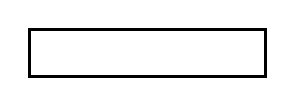
\begin{tikzpicture}
\def\a{.3}
\FixedSupport[-90]{0,\a}{1.5}
\draw[very thick](0,0)rectangle(3,2*\a);
\NodalForce{5,\a}[G][N][N]
\NodalForce{7,\a}[Q][N][N]
\end{tikzpicture}
\end{figure}
\end{exmp}
\begin{solution}
The resistance against axial tension yield is
\begin{gather*}
R=A_gf_y=\dfrac{\pi{}d^2}{4}f_y.
\end{gather*}
\begin{itemize}
\item \textbf{ASD}\\
Allowable force: $R/\mathrm{SF}=A_gf_y/\num{1.7}$. Working forces: $\sum{}E_i=G+Q=\SI{55}{\kn}$.\\
ASD requires:
\begin{align*}
\sum{}E_i&\leqslant{}R/\mathrm{SF}\\
\SI{55}{\kn}&\leqslant\dfrac{\pi{}d^2}{4\times1.7}f_y\\
d&\geqslant\sqrt{\dfrac{\SI{55}{\kn}\times4\times1.7}{\SI{300}{\mpa}\times\pi}}=\SI{19.9}{\mm}
\end{align*}
\item \textbf{LRFD}\\
LRFD requires:
\begin{align*}
\gamma_GE_G+\gamma_QE_Q&\leqslant\phi{}R\\
1.2\times\SI{25}{\kn}+1.5\times\SI{30}{\kn}&\leqslant0.9\times\dfrac{\pi{}d^2}{4}f_y\\
d&\geqslant\sqrt{\dfrac{\SI{75}{\kn}\times4}{0.9\times\SI{300}{\mpa}\times\pi}}=\SI{18.8}{\mm}
\end{align*}
\end{itemize}
If rods come in \SI{2}{\mm} size increments, then in both cases a $\phi~\SI{20}{\mm}$ rod is OK.
\end{solution}
\clearpage
For handwritten homework, please follow the convention as shown in the example.
\begin{figure}[H]
\centering
\includegraphics[width=.99\textwidth]{PIC/CH01/SAMPLE}
\caption{Sample handwritten solution}
\end{figure}
\section{Calculation Accuracy}
Estimates of likely maximum forces (or actions) and resistances are generally very approximate in design. Also, the load factors and resistance factors are not provided with great precision. For this reason, using more than three significant digits is seldom necessary and three significant digits is generally used. (Care must be taken though because in some cases, such as when similar size numbers are subtracted more accuracy is required.)

Because the computed result contains a lot of uncertainty, it may not be necessary to follow the calculation results too rigidly. However, because we may need to defend our calculations in a court of law, we must make sure that our recommendations, based on our calculations are totally defensible.

Gregory MacRae suggests the following guidelines:
\begin{itemize}
\item If the demand is greater than the capacity by \textbf{less than 1\%}, then the difference is usually within the range of usual round-off errors. It can usually be argued that greater than nominal material strengths and strain hardening will guarantee that the demand is greater than the capacity. A note of this sort should be made in the calculations.
\item If the demand is greater than the capacity by \textbf{less than 5\%}, then the design should only be accepted if it can be argued that the design is satisfactory for some reason which is not considered in the calculations used in the design approach. The reason for accepting the design should be stated in the calculations, and the engineer should be able to produce more refined calculations to justify the decision if required at a later date.
\item If the demand is greater than the capacity by \textbf{more than 5\%}, then the design should not be accepted, or a revised set of calculations should be carried out to show that the design works.
\end{itemize}
It should be noted that different groups have different approaches to accuracy and it is prudent to check the policy of the company you are working for.